\section{Cơ sở lý thuyết}
\subsection{Phương pháp áp dụng - KGAT}
\subsection{Phương pháp khác}
\subsubsection{Content-based Filtering}
\subsubsection{Matrix Factorization - Bayesian Personalized Ranking}
\subsubsection{Factorization Machine}
Một trong những nhược điểm chính của mô hình BPRMF là không có khả năng mô hình hóa 
những thông tin bổ trợ giữa người dùng và sản phẩm. Do đó, một phương pháp mở rộng FM đã ra đời. 
Đây cũng là phương pháp nền móng cho các kĩ thuật DL được ra đời cho bài toán khuyến nghị.
\newline
\indent Thuật toán khuyến nghị FM có thể mở rộng ra với các thông tin bổ trợ của người dùng và sản phẩm. 
Ví dụ như về khuyến nghị cho người dùng một bộ phim, ta có thể xét mức độ ảnh hưởng của 
các thông tin bổ trợ như: giới tính, tuổi, nghề nghiệp, ... Những thành phần này sẽ được mã hóa 
thành các vector one-hot hoặc multi-hot vector. Nếu có thêm các dữ liệu dạng số khác, 
ta có thể thêm vào $\mathbf{x}$ các thành phần tương ứng. Với mỗi thành phần được thêm vào 
$\mathbf{x}$, ta thêm một cột vector embedding vào $\mathbf{V}$ như hình bên dưới đây.
Khi đó, độ quan tâm của người dùng có thể được dựng lên như sau:

$$\hat{y}_{ij} = w_0 + \mathbf{xw} + \sum_{i=1}^{d}\sum_{j=i+1}^{d} \mathbf{v}_i^T\mathbf{v}_jx_ix_j$$

Trong đó:

\begin{itemize}
    \item $\mathbf{w_0}$ đóng vai trò như một hệ số bias trong mô hình hồi quy tuyến tính, 
    nó có thể được xem như là một hệ số vô hướng cố định thêm vào kết quả dự đoán cuối cùng để điều chỉnh sự lệch trung bình.
    \item $\mathbf{xw}$: đây là tích vô hướng vector đặc trưng đầu vào (input feature vector) 
    và một vector trọng số $\mathbf{w}$ tương ứng với các đặc trưng của $\mathbf{x}$.
    \item $\sum_{i=1}^{d}\sum_{j=i+1}^{d} \mathbf{v}_i^T\mathbf{v}_jx_ix_j$: Đây là thành phần tương tác bậc hai giữa các đặc trưng.
    \begin{itemize}
        \item $x_i$, $x_j$ lần lượt là phần tử thứ $i$, thứ $j$ trong feature vector $\mathbf{x}$.
        \item $\mathbf{v}_i^T\mathbf{v}_j$ là tích vô hướng giữa các vector embeddings tương ứng với từng đặc trưng đầu vào $x_i$ và $x_j$.
        \item $\sum_{i=1}^{d}\sum_{j=i+1}^{d} \mathbf{v}_i^T\mathbf{v}_jx_ix_j$ là biểu diễn tổng tất cả các cặp tương tác giữa các đặc trưng có trong tập dữ liệu.    
    \end{itemize}
\end{itemize}

Đây chính là ý tưởng chính của FM. Đồng thời, nhờ vào việc $\mathbf{x}$ thường là một vector rất thưa (rất ít thành phần khác 0), 
việc huấn luyện và dự đoán trở nên rất nhanh ngay cả khi số lượng người dùng và sản phẩm lớn.

\subsubsection{Neutral Factorization Machine}
Mặc dù có khả năng mô hình hóa các thông tin bổ trợ của người dùng và sản phẩm, performance của FM vẫn bị hạn chế 
bởi tính tuyến tính của nó cũng như việc chỉ mô hình các tương tác đặc trưng (ví dụ như bậc 2) theo cặp. 
Với dữ liệu thực tế có cấu trúc cơ bản phức tạp và phi tuyến, FM sẽ không đủ khả năng biểu diễn. 
Tuy FM bậc cao hơn đã được đề xuất, chúng vẫn thuộc họ mô hình tuyến tính và được cho là khó ước tính.

\indent NFM ra đời nhằm cải tiến FM bằng cách mô hình hóa các tương tác đặc trưng cao và phi tuyến. 
Bằng cách sử dụng một phép toán mới trong mô hình neural network - Bilinear Interaction (Bi-interaction) pooling, 
NFM được xem như là sự kết hợp của FM với neural network framework. Thông qua việc xếp chồng các lớp phi tuyến trên Bi-interaction pooling layer, 
NFM đã làm sâu hơn mô hình FM tuyến tính nông, từ đó mô hình hóa các tương tác đặc trưng phi tuyến và bậc cao một cách hiệu quả, cải thiện performance của FM.

\indent Với một feature vector thưa $\mathbf{x} \in \mathbb{R}^{n}$ làm đầu vào, trong đó $x_i = 0$ nghĩa là đặc trưng thứ $i$ không tồn tại trong đối tượng, 
NFM dự đoán mục tiêu như sau:
$$ \hat{y}(\mathbf{x}) = w_0 + \mathbf{xw} + f(\mathbf{x})$$

Trong đó, term đầu tiên và thứ 2 là phần linear regression giống với FM, 
thứ mô hình bias toàn cục và trọng số của các đặc trưng. Còn term thứ 3 $f(\mathbf{x})$ là thành phần cốt lõi trong NFM 
để mô hình tương tác đặc trưng. $f(\mathbf{x})$ chính là một multi-layer feed-forward neural network như bên dưới:
\begin{figure}[h]
    \centering
    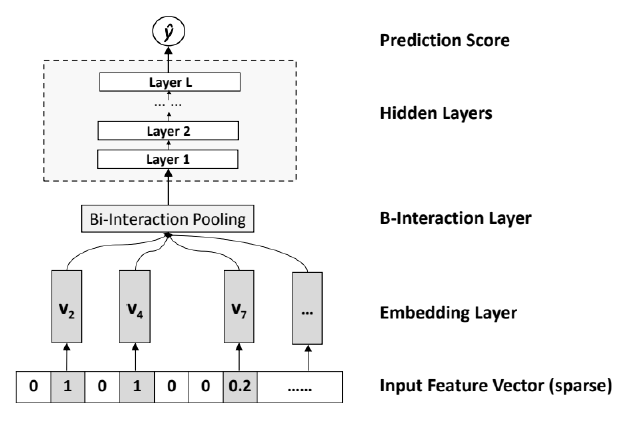
\includegraphics[width=0.7\linewidth]{figures/63.png}
\end{figure}\\
Do Embedding layer tương tự như FM nên ta sẽ tiếp tục tìm hiểu về Bi-Interaction pooling, Hidden layer, Prediction layer.

\textbf{Bi-interaction pooling:} chuyển đổi tất các embedding vectors $V_x$ thành 1 vector như sau:
$$ f_{BI}(V_x) = \sum_{i=1}^{n} \sum_{j=i+1}^{n} x_i v_i \odot x_j v_j $$
Trong đó, $\odot$ là ký hiệu của element-wise product của 2 vectors; $x_i$, $x_j$ lần lượt 
là phần tử thứ $i$ và $j$ trong feature vector $\mathbf{x}$. $\mathbf{v}_i, \mathbf{v}_j$ lần lượt là embedding của feature thứ $i$ và $j$.
\textbf{Hidden layer:} Trên Bi-interaction pooling là 1 chồng các lớp fully connected, thứ có khả năng mô hình các tương tác bậc cao giữa các đặc trưng. 
Mỗi hidden layer sẽ có một non-linear activation function như tanh, sigmoid, ReLU.
\textbf{Prediction layer:} Cuối cùng, vector đầu ra của hidden layer cuối sẽ được chuyển đổi thành prediction score:
$$f(\mathbf{x}) = \mathbf{h}^T \mathbf{z}_L$$
Trong đó, $\mathbf{h}$ là weight của prediction layer, $\mathbf{z}_L$ là output vector của hidden layer cuối.
